\begin{center}
     \Large{\textbf{AND Cheat Sheet}} \\
\end{center}

\section{Vocabulary}
\textsc{Hyperbolic eq.points} $\Re\{\lambda\} \neq 0$ \\
\textsc{Nonhyperbolic problems} Equilibria with EV on the imaginary axis.

\section{Basics on cont.-time dynamical systems}
\begin{align*}
\dot{x} = f(t,x,p), \quad x(t_0) = x_0 \Leftrightarrow \dx = f(x,p), \quad x(0)=x_0
\end{align*}
\subsection{Flow of a system}
Solution is the flow $\phi_t(x_0)$
\begin{align*}
x(t;x_0,p)=\phi_t(x_0,p)
\end{align*}
\textsc{Flow axioms}\\
\begin{align*}
\phi_0(x_0,p)&=x_0\\
\phi_{t_1}[\phi_{t_2}(x_0,p),p] &= \phi_{t_1+t_2}(x_0,p)
\end{align*}
\subsection{Existence and uniqueness}
\textsc{Existence and uniqueness of local (in time) solutions}\\
\emph{If $f(x)$ is smooth enough, then solutions exist and are unique. No guarantee that they exist forever - only guarantees to exist in a very short time interval around $t_0$.}\\
If $f$ is Lipschitz in $x$ and piecewise continuous in $t$ then the IVP has a unique solution $x(t)=\phi(t;t_0)x_0$ over a finite time interval $t\in[t_0-\tau,t_0+\tau]$.\\
Allows for finite-escape times/blow-up (reach infinity in finite time).

\subsection{Stability}
Def.: An equilibrium point is a state $x^*$ s.t. $f(x^*)=0$\\
Def.: An eq.point $x^*$ is stable if for any $\epsilon>0$ there exists a constant $\delta > 0$ such that \begin{align*}
\forall x_0: \Vert x_0 - x^* \Vert \leq \delta \Rightarrow \Vert x(t)-x^* \Vert \leq \epsilon \quad \forall t \geq 0
\end{align*}

\textsc{Attractor}\\
$x^*$ is attractive if $\lim_{t\rightarrow \infty} \Vert x(t)-x^* \Vert = 0 \quad \forall x_0 \in \mathcal{S}$ with $\mathcal{S}$ being the domain of attraction.\\
Eq points may be attractive without being stable (ex. Vinograd's system).

\textsc{Asymptotic stability}\\
An eq.point $x^*$ is asymptotically stable if it is stable and attractive.

\textsc{Exponential stability}\\
An eq.point $x^*$ is exponentially stable in $\mathcal{S}$ if it is stable and there are constants $a, \lambda > 0$ such that $\forall x_0 \in \mathcal{S}: \Vert x(t)-x^*\Vert \leq a\Vert x_0 - x^* \Vert e^{-\lambda t}$

\section{Linear systems}
\subsection{LTI Systems}
\[ \dot{x} = f(x,u) \rightarrow \dot{x} = Ax \]
mit $A \in \mathbb{R}^{n \times n}$ linear map/transformation

Theorem:
The origin of the linear system is stable if all EV $\lambda_i$ have non positive real part. If all EV have negative Real part, the origin is exponentially stable.

\[ \lambda^2+tr(A)\lambda+det(A) = 0 \]
\[ tr(A) = a_{11} + a_{22} \]
\[ det(A) = a_{11}a_{22} - a_{12}a_{21} \]

\[ \lambda_{1,2} = \frac{1}{2} (tr(A) \pm \sqrt{tr(A)^2-4det(A)} \]

daraus folgt
$tr(A) < 0 \rightarrow$ stable\\
$tr(A) > 0 \rightarrow$ unstable\\
$tr(A)^2 \geq 4det(A)$ node\\
$tr(A)^2 < 4det(A)$ spiral\\

Spezialfall:
$tr(A)^2 = 4det(A)$ $\rightarrow$ stable if $tr(A) < 0$ and if $det(A) < 0 \rightarrow$ saddle


%\begin{pspicture}(6,5)
%    \psline{->}(0,2)(5,2) \rput*(5.5,2){det}
%    \psline{->}(2,0)(2,4) \rput*(2,4.2){tr}
%    \rput(3.2,4){unstable node}
%    \rput(3.5,2.5){unstable spiral}
%    \rput(3.5,1.5){stable spiral}
%    \rput(3,0.5){stable node}
%    \rput(0.5,2.5){saddles}
%    \rput(0.5,1.5){saddles}
%    \pscurve(4.5,3.5)(2,2)(4.5,0.5)
%\end{pspicture}

\subsection{LTV Systems and Floquet theory}

\subsubsection{Local Nonlinear Flows}
\textsc{Hartman-Grobman Theorem}\\
The local phase portrait of the linearization (stability) of the fixed point is captured by the linearization. (for hyperbolic fixed points)
\emph{Hyperbolic}: $EV of J(x^*,p) \neq 0$

\subsubsection{Center Manifold theorem}
\[ \frac{dh}{dx_z} [A_z x_z + f_z(x_z,h(x_z))] = A_s h(x_z) + f_s(h(x_z),x_y) \]
\[ h(0) = 0, \frac{dh(0)}{dx_z} = 0 \]

\subsubsection{Index theory}
Fuer mehr globale information\\
stable, unstable node $I_C = -1$\\
s/u spiral $I_C = 1$\\
s/u limit cycle $I_C = 1 \rightarrow$ wegen EP im Kern
\subsubsection{Limit Cycles}
Isolated (no other closed trajectory, spiral towards or away from LC) closed trajectories

\textsc{Poincare Bendixson}\\
\subsection{Local Theory}
\textsc{Hartman-Grobman}\\
The behavior of a nonlinear systems in a vicinity of hyperbolic eq. points is the same as in the linearized system around that point.

\textsc{Center manifold theorem}\\
\begin{align*}
\frac{dh}{dx_z}[A_zx_z+f_z(x_z, h(x_z))] = A_sh(x_z)+f_s(h(x_z),x_z) \\
h(0)=0, \quad \frac{dh(0)}{dx_z} = 0
\end{align*}


\subsection{Non-local phenomena}
\section{Bifurcations of vector fields}
\subsection{Bifurcations of SSs}
\textsc{Transcritical bifurcation}\\
\emph{Standard mechanism for change of stability for a fixed point which exists for all values of the parameter}.\\
Ex.: $\dot{x}=rx-x^2$.\\
Fixed point at $x^*=0 \quad \forall r$. For $r<0$ unstable fixed point at $x^*=r$ and a stable at $x^*=0$. For $r=0^-$ the fixed points unify. For $r>0$ the origin is unstable and $x^*=r$ becomes stable - \textbf{exchange of stabilities}
\begin{center}
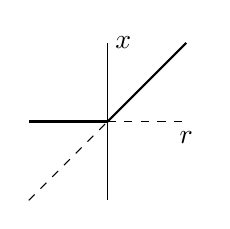
\begin{tikzpicture}
\draw (0,1.5) -- (0,-0.5);
\draw [thick](-1,0.5) -- (0,0.5);
\draw [dashed](0,0.5) -- (1,0.5);
\draw [thick](0,0.5) -- (1,1.5);
\draw [dashed](-1,-0.5) -- (0,0.5);
\node at (1,0.3) {$r$};
\node at (0.2,1.5) {$x$};
\end{tikzpicture}
\end{center}
\vspace{0.2cm}


\textsc{Saddle node bifurcation}\\
\emph{Fixed points are created and destroyed. As a parameter is varied, two fixed points move toward each other, collide and mutually annihilate}.\\
Ex: $\dot{x}=r+x^2$.\\ $r<0$: 2 FP (1 stable, 1 unstable),\\ $r=0^-$: half-stable FP, \\ $r>0$: no FP.\\ In this example the bifurcation occurred at $r=0$.
\begin{center}
\begin{tikzpicture}
\draw (0,1.5) -- (0,-0.5);
\draw (-1,0.5) -- (1,0.5);
\draw [thick](-1,-0.25) .. controls (-0.5,-0.1) and (0,0) .. (0,0.5);
\draw [dashed](-1,1.25) .. controls (-0.5,1.1) and (0,1) .. (0,0.5);
\node at (1,0.3) {$r$};
\node at (0.2,1.5) {$x$};
\end{tikzpicture}
\end{center}
\vspace{0.2cm}

\subsubsection{Pitchfork bifurcation}
\emph{Common in physical systems that have (left/right) symmetry.}
\textsc{Supercritical pitchfork bifurcation}\\
Ex: $\dot{x}=rx-x^3$. If $r<0$ the origin is the only fixed point and stable. $r=0$ the origin is still stable, but weakly, since the linearization vanishes (solutions no longer decay exponentially fast - \emph{critical slowing down}).  For $r>0$ the origin becomes unstable and two new stable fixed points appear at $x^*=\pm \sqrt{r}$.
\begin{center}
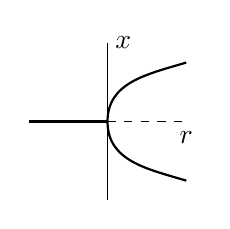
\begin{tikzpicture}
\draw (0,1.5) -- (0,-0.5);
\draw [thick](-1,0.5) -- (0,0.5);
\draw [dashed](0,0.5) -- (1,0.5);
\draw [thick](1,-0.25) .. controls (0.5,-0.1) and (0,0) .. (0,0.5);
\draw [thick](1,1.25) .. controls (0.5,1.1) and (0,1) .. (0,0.5);
\node at (1,0.3) {$r$};
\node at (0.2,1.5) {$x$};
\end{tikzpicture}
\end{center}
\vspace{0.2cm}

\textsc{Subcritical pitchfork bifurcation}\\
Ex: $\dot{x}=rx+x^3$. Only for $r<0$ two unstable fixed points $x^*=\pm \sqrt{-r}$ and stable origin. For $r>0$ origin is unstable (finite escape)
\begin{center}
\begin{tikzpicture}
\draw (0,1.5) -- (0,-0.5);
\draw [thick](-1,0.5) -- (0,0.5);
\draw [dashed](0,0.5) -- (1,0.5);
\draw [dashed](-1,-0.25) .. controls (-0.5,-0.1) and (0,0) .. (0,0.5);
\draw [dashed](-1,1.25) .. controls (-0.5,1.1) and (0,1) .. (0,0.5);
\node at (1,0.3) {$r$};
\node at (0.2,1.5) {$x$};
\end{tikzpicture}
\end{center}

\subsubsection{Bifurcations of SSs in dim $n>1$}
\begin{align*}
\text{transcritical bif: }& \dot{x}_1=rx_1-x_1^2 \quad &\dot{x}_2 = \pm x_2 \\
\text{saddle-node bif: }& \dot{x}_1 = r-x_1^2, \quad &\dot{x}_2 = \pm x_2\\
\text{pitchfork bif: }& \dot{x}_1=rx_1-x_1^3, \quad &\dot{x}_2 = \pm x_2
\end{align*}

\subsection{Bifurcations of trajectories}
\textsc{Flows on the circle}\\
Vector field on the circle $\dot{\Theta}=f(\Theta)$, with $\Theta$ being a point on the circle. Particle can return to starting place - most basic model of oscillating systems.\\

\textsc{Non-uniform oscillator}\\
$\dot{\Theta} = \omega - a\sin \Theta$ with mean $\omega$ and amplitude $a$.\\
\textbf{Uniform oscillator $p=0$}: $\dot{\Theta} = \omega$ and $\omega=\text{const.}$ with solution $\Theta(t)=\omega t + \Theta_0$. \emph{Phase $\Theta$ changes uniformly}.\\
\begin{center}
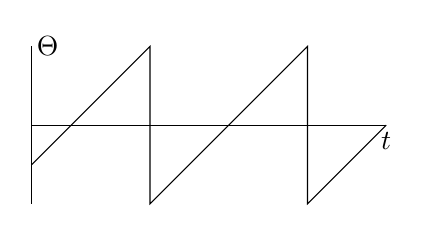
\begin{tikzpicture}
\draw (-1,1.5) -- (-1,-0.5);
\draw (-1,0.5) -- (3.5,0.5);
\node at (3.5,0.3) {$t$};
\node at (-0.8,1.5) {$\Theta$};
\draw (-1,0) -- (0.5,1.5) -- (0.5,-0.5) -- (2.5,1.5) -- (2.5,-0.5) -- (3.5,0.5);
\end{tikzpicture}
\end{center}

For $0<p<\omega$ there is a non uniform oscillation, because the velocity depends on the angle. For $p=\omega$ a SS appears at $\Theta=\sfrac{\pi}{2}$ attracting the flow from one side and repelling the other side. For $p>\omega$ there are two SSs (1 repulsor, 1 attractor).\\
For $p\lesssim\omega$ there exists a saddle-note ghost. Time to pass through the bottleneck via local rescaling around the bottleneck: $\dot{x}=r+x^2$ where $0<r = \frac{2(\omega-a)}{a}\ll 1$ is proportional to the distance of the bif. $T\approx
\int_{-\infty}^{\infty} \frac{dx}{r+x^2} = \frac{\pi}{\sqrt{r}}$

\begin{center}
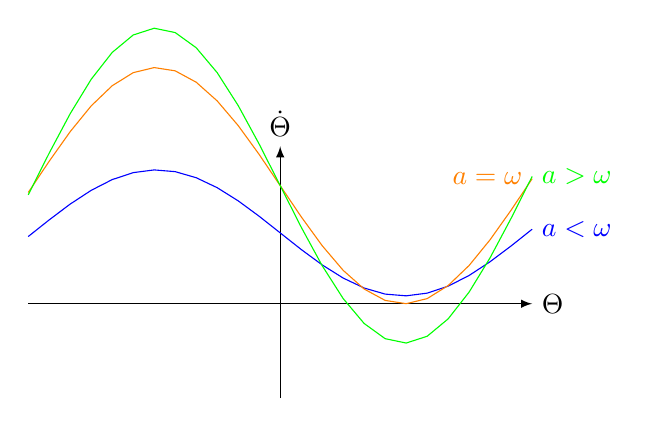
\begin{tikzpicture}[domain=-3.2:3.2]
\draw[-latex] (-3.2,0) -- (3.2,0) node[right] {$\Theta$};
\draw[-latex] (0,-1.2) -- (0,2) node[above] {$\dot{\Theta}$};
\draw[color=blue] plot (\x,{0.9-0.8*sin(\x r)}) node[right] {$a<\omega$};
\draw[color=orange] plot (\x,{1.5-1.5*sin(\x r)}) node[left] {$a=\omega$};
\draw[color=green] plot (\x,{1.5-2*sin(\x r)}) node[right] {$a>\omega$};
\end{tikzpicture}   
\end{center}

\subsubsection{Andronov-Hopf bifurcation (2D)}
\emph{No SSs appear/disappear. Rather the behaviour changes qualitatively for small variations, e.g. decaying oscillation vs. increasing oscillation with limiting amplitude after the bifurcation.}\\
Can occur in phase spaces of any dimension $n\geq 2$.

\textsc{Supercritical Hopf bifurcation}\\
Decay rate dependent on control parameter $p$. Decay becomes slower and slower and finally changes to a growth at a critical $p_c$ (equilibrium becomes unstable). In many cases there results a limit cycle about the former SS. \textbf{In phase plane:} Stable spiral becomes unstable spiral surrounded by a small nearly elliptical limit cycle.
Example:
\begin{align*}
\dot{r}=pr-r^3\\
\dot{\Theta}=\omega+br^2
\end{align*}
with control parameter $p$, $\omega$ frequency and $b$ as dependence of frequency on amplitude. Stable spiral for $p<0$ in origin $r=0$ and sense of rotation depends on $\omega$. For $p=0$ the origin is very weakly stable. For $p>0$ there is an unstable spiral at the origin and a stable limit cycle at $r=\sqrt{p}$.\\
EV analysis via cartesian coordinates $x_1=r\cos \Theta$, $\;x_2=r\sin \Theta$ yields $\dot{x}_1 = px_1-\omega x_2$, $\quad\dot{x}_2 = \omega x_1+p x_2$ with the Jacobian $J=\begin{bmatrix}
p & -\omega \\ \omega & p
\end{bmatrix}$ and $\lambda_{1,2} = p \pm i\omega$. EVs cross the imaginary axis from left to right as $p$ increases from - to +. \\
\textbf{Rules of thumb:} Size of limit cycle grows from 0 proportionally to $\sqrt{p-p_c}$. Frequency of limit cycle $\omega \approx \Im \{\lambda\}$ evaluated at $p=p_c$.
\begin{center}
\begin{tikzpicture}
\draw (0,1.5) -- (0,-0.5);
\draw [thick](-1,0.5) -- (0,0.5);
\draw [thick,dashed](0,0.5) -- (1,0.5);
\draw [line width=2, line cap=round, dash pattern=on 0pt off 2\pgflinewidth] (1,1.25) .. controls (0.5,1.1) and (0,1) .. (0,0.5);
\node at (1,0.3) {$p$};
\node at (0.2,1.5) {$r$};
\end{tikzpicture}
\end{center}
\vspace{0.2cm}

\textsc{Subcritical Hopf bifurcation (More Dangerous)}\\
\emph{Stable origin surrounded by unstable limit cycle which collapses at $p=0$ leading to a repulsive spiral with no saving limit cycle around.}\\
Example:
\begin{align*}
\dot{r}=pr+r^3\\
\dot{\Theta}=\omega+br^2
\end{align*}
Cubic term is destabilizing yielding a stable origin and a unstable unstable limit cycle at $r=-\sqrt{-p}$ only existing for $p<0$. Unstable for $p\geq 0$ (weakly at $p=0$).
\begin{center}
\begin{tikzpicture}
\draw (0,1.5) -- (0,-0.5);
\draw [thick](-1,0.5) -- (0,0.5);
\draw [thick,dashed](0,0.5) -- (1,0.5);
\draw [line width=2.1, line cap=round, dash pattern=on 0pt off 2\pgflinewidth](-1,1.25) .. controls (-0.5,1.1) and (0,1) .. (0,0.5);
\draw [color=white,line width=2.1, line cap=round, dash pattern=on 0pt off 2\pgflinewidth](-1,1.25) .. controls (-0.5,1.1) and (0,1) .. (0,0.5);
\node at (1,0.3) {$p$};
\node at (0.2,1.5) {$r$};
\end{tikzpicture}
\end{center}
\vspace{0.2cm}

\textsc{Degenerate Hopf bifurcation}\\
\emph{Conj. complex EV pass through the imaginary axis, but do not isolated periodic orbits (limit cycle).}\\
Linear system example:
\begin{align*}
\dot{x}_1=px_1-x_2\\
\dot{x}_2=x_1+px_2\\
\end{align*}
Nonlinear example, inverted pendulum with Coulomb friction $\ddot{\Theta}+\rho \dot{\Theta} + k\sin \Theta = 0$. For $p<0$ stable spiral, a center (\emph{no limit cycles}) for $p=0$ (band of closed orbits) and unstable spiral for $p>0$.

\subsubsection{Bifurcation of limit cycles}
\textsc{Infinite period bifurcation}\\
Example:
\begin{align*}
\dot{r}=r-r^2\\
\dot{\Theta}=p-\Theta^2
\end{align*}
Two radial equilibrium solutions $r=0$ and $r=1$ (attractive). For $p<0$ no angular eq.point exists so that the limit cycle $r=1$ is a unique attractor, attracting trajectories from unstable origin. For $p=0$ a SS at $(r,\Theta)=(1,0)$ appears similar to a saddle point with radial attraction ($x_1$-direction) and angular saddle behaviour - the time through the bottleneck of $p<0$ becomes infinite for $p=0$. For $p>0$ there are two SSs at $(1,\sqrt{p})$ (attractor) and $(1,-\sqrt{p})$ (repulsor) - looks like pacman.
\begin{center}
\begin{tikzpicture}
\draw (0,1.5) -- (0,-0.5);
\draw [thick,dashed](-1,0.5) -- (0,0.5);
\draw [thick,dashed](0,0.5) -- (1,0.5);
\draw [line width=2.1, line cap=round, dash pattern=on 0pt off 2\pgflinewidth](-1,1) -- (0,1);
\draw [color=white,line width=2.1, line cap=round, dash pattern=on 0pt off 2\pgflinewidth](-1,1) -- (0,1);
\draw [thick](0,1) -- (1,1);
\node at (1,0.3) {$p$};
\node at (0.2,1.5) {$r$};
\end{tikzpicture}
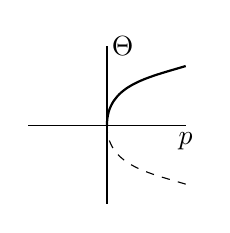
\begin{tikzpicture}
\draw (0,1.5) -- (0,-0.5);
\draw (-1,0.5) -- (0,0.5);
\draw (0,0.5) -- (1,0.5);
\draw [dashed](1,-0.25) .. controls (0.5,-0.1) and (0,0) .. (0,0.5);
\draw [thick](1,1.25) .. controls (0.5,1.1) and (0,1) .. (0,0.5);
\node at (1,0.3) {$p$};
\node at (0.2,1.5) {$\Theta$};
\end{tikzpicture}
\end{center}

\textsc{Saddle-node bifurcation of cycles}\\
